%FOR PDFLATEX USE ONLY
\documentclass[a4paper,12pt]{article}

\usepackage{amssymb,amsmath} %math symbols

\usepackage[margin=2cm]{geometry} %paper geometry

\usepackage[utf8]{inputenc} %allows unicode (including russian) source file
\usepackage[russian]{babel} %docment in russian-style
\usepackage[utf8]{inputenc}
\usepackage[unicode]{hyperref} %links inside of the text
\usepackage[pdftex]{graphicx} %includegraphics pictures
\usepackage{cmlgc} %bold text

\usepackage{array} %arrays

\usepackage{wrapfig}
\usepackage{array}
\usepackage{lipsum}
\usepackage{esvect}
\usepackage{hyperref}
\usepackage{xcolor}
\definecolor{linkcolor}{HTML}{799B03} % цвет ссылок
\definecolor{urlcolor}{HTML}{799B03} % цвет гиперссылок
 
\hypersetup{pdfstartview=FitH,  linkcolor=linkcolor,urlcolor=urlcolor, colorlinks=true}
 
\usepackage{subfig}
\usepackage{calc}
\usepackage{pgfplots,tikz,circuitikz}
\usepackage{pgfplotstable}
\usepackage{tkz-euclide}

\usepackage{centernot}
\usepackage{cancel}

\documentclass{article}
\usepackage{amsmath}
\usepackage{mathtext}
\usepackage[T1,T2a]{fontenc}
\usepackage[utf8]{inputenc}
\usepackage[english, bulgarian, russian]{babel}
\usepackage{tikz}
\usepackage{pgfplots}
\usepackage[export]{adjustbox}
\usepackage[left=2cm,right=2cm,
    top=2cm,bottom=2cm,bindingoffset=0cm]{geometry}

\usepackage{csvsimple}

\begin{document}

\begin{center}
  \LARGE{Работа 2.1.6}\\[0.2cm]
  \LARGE{Эффект Джоуля–Томсона.}\\[0.2cm]
  \large{Панферов Андрей}\\[0.2cm]
\end{center}


\textbf{Цель работы:} определение изменения температуры углекислого газа при протекании через малопроницаемую перегородку при разных начальных значениях давления и температуры; 2) вычисление по результатам опытов коэффициентов Ван-дер-Ваальса «a» и «b».

\textbf{В работе используются:} трубка с пористой перегородкой; труба Дьюара; термостат; термометры; дифференциальная термопара; микровольтметр; балластный баллон; манометр.

\textbf{Теоретическаие сведения}

Эффектом Джоуля–Томсона называется изменение температуры газа, медленно протекающего из области высокого в область низкого давления в условиях хорошей тепловой изоляции. В разреженных газах, которые приближаются по своим свойствам к идеальному газу, при таком течении температура газа не меняется. Эффект Джоуля–Томсона демонстрирует отличие исследуемого газа от идеального.\\

\begin{figure}[h!]
\centering{
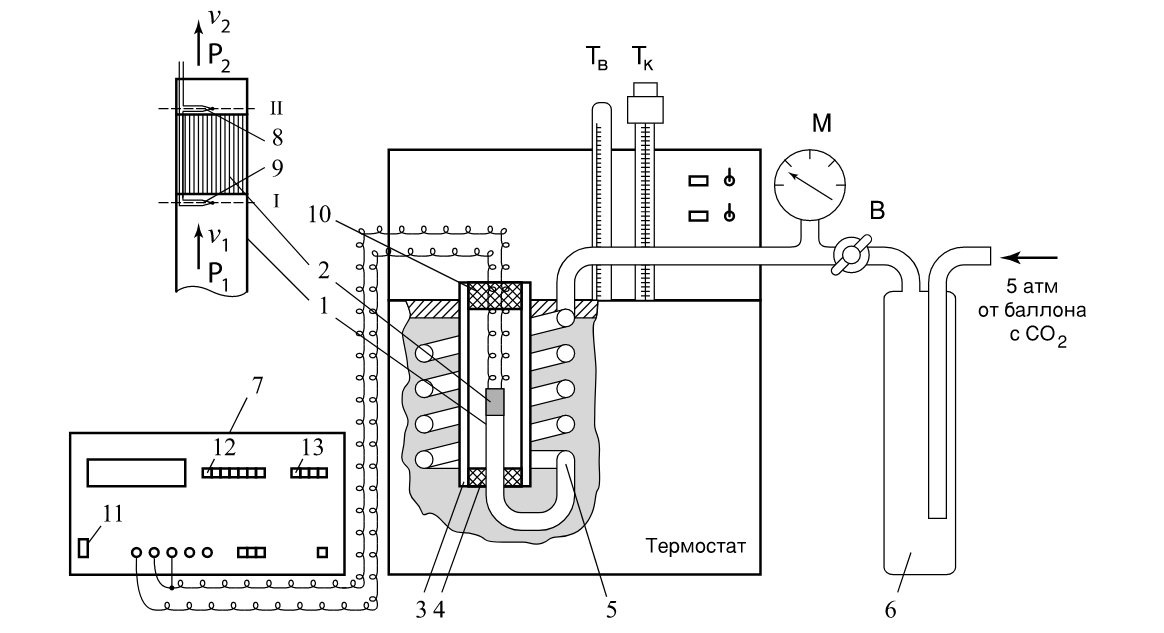
\includegraphics[width=15cm]{scheme.png}
}
\caption{Схема установки для изучения эффекта Джоуля–Томсона.}
\end{figure}

В работе исследуется изменение температуры углекислого газа при медленном его течении по трубке с пористой перегородкой (рис. 1). Трубка 1 хорошо теплоизолирована. Газ из области повышенного давления $P_1$ проходит через множество узких и длинных каналов пористой перегородки 2 в область с атмосферным давлением $P_2$. Перепад давления $\Delta P = P_1 - P_2$ из-за большого сопротивления каналов может быть заметным даже при малой скорости течения газа в трубке. Величина эффекта Джоуля–Томсона определяется по разности температуры газа до и после перегородки.\\

Рассмотрим стационарный поток газа между произвольными сечениями I и II трубки (до перегородки и после нее). Пусть, для определенности, через трубку прошел 1 моль углекислого газа; $\mu$ --- его молярная масса. Молярные объемы газа, его давления и отнесенные к молю внутренние энергии газа в сечениях I и II обозначим соответственно $V_1, P_1, U_1$ и $V_2, P_2, U_2$. Для того чтобы ввести в трубку объем $V_1$, над газом нужно совершить работу $A_1 = P_1V_1$. Проходя через сечение II, газ сам совершает работу $A_2 = P_2V_2$. Так как через боковые стенки не происходит ни обмена теплом, ни передачи механической энергии, то:

\begin{equation}
A_1 - A_2 = \left(U_2 + \dfrac{\mu v_2^2}{2}\right) - \left(U_1 + \dfrac{\mu v_1^2}{2}\right).
\end{equation}

В уравнении (1) учтено изменение как внутренней (первые члены в скобках), так и кинетической (вторые члены в скобках) энергии газа. Подставляя в (1) написанные выражения для $A_1$ и $A_2$ и перегрупп ровывая члены, найдем:

\begin{equation}
H_1 - H_2 = (U_1 + P_1V_1) - (U_2 + P_2V_2) = \dfrac{1}{2} \mu (v_2^2 - v_1^2).
\end{equation}

Сделаем несколько замечаний. Прежде всего отметим, что в процессе Джоуля–Томсона газ испытывает в пористой перегородке суще- ственное трение, приводящее к ее нагреву. Потери энергии на нагрев трубки в начале процесса могут быть очень существенными и сильно искажают ход явления. После того как температура трубки установится и газ станет уносить с собой все выделенное им в пробке тепло, формула (1) становится точной, если, конечно, теплоизоляция трубки достаточно хороша и не происходит утечек тепла наружу через ее стенки.\\

Второе замечание связано с правой частью (2). Процесс Джоуля–Томсона в чистом виде осуществляется лишь в том случае, если правой частью можно пренебречь, т. е. если макроскопическая скорость газа с обеих сторон трубки достаточно мала. У нас сейчас нет критерия, который позволил бы установить, когда это можно сделать. Поэтому мы отложим на некоторое время обсуждение вопроса о правой части (2), а пока будем считать, что энтальпия газа не ме- няется.

\begin{equation}
\mu_{Д-Т} = \dfrac{\Delta T}{\Delta P} \approx \dfrac{\frac{2a}{RT}-b}{C_p}.
\end{equation}

Отсюда видно, что эффект Джоуля–Томсона для не очень плотного газа зависит от соотношения величин $a$ и $b$, которые оказывают противоположное влияние на знак эффекта. Если силы взаимодействия между молекулами велики, так что превалирует <<поправка на давление>>, то основную роль играет член, содержащий $a$, и

\begin{equation}
$$\dfrac{\Delta T}{\Delta P} > 0,$$
\end{equation}

то есть газ при расширении охлаждается ($\Delta T < 0$, так как всегда $\Delta P < 0$). В обратном случае (малые $a$)

\begin{equation}
\dfrac{\Delta T}{\Delta P} < 0,$$
\end{equation}

то есть газ нагревается ($\Delta T > 0$, так как по-прежнему $\Delta P < 0$).\\

Этот результат нетрудно понять из энергетических соображений. Как мы уже знаем, у идеального газа эффект Джоуля–Томсона отсутствует. Идеальный газ отличается от реального тем, что в нем можно пренебречь потенциальной энергией взаимодействия молекул. Наличие этой энергии приводит к охлаждению или нагреванию реальных газов при расширении. При больших $a$ велика энергия притяжения молекул. Это означает, что потенциальная энергия молекул при их сближении уменьшается, а при удалении --- при расширении газа --- возрастает. Возрастание потенциальной энергии молекул происходит за счет их кинетической энергии --- температура газа при расширении падает. Аналогичные рассуждения позволяют понять, почему расширяющийся газ нагревается при больших значениях $b$.\\

Как следует из формул (1.35), (1.36), при температуре $T_i$ коэффициент $\mu_{Д-Т} $ обращается в нуль. Используя связь между коэффициентами $a$ и $b$ и критической температурой (1.19), по формуле (1.36) найдем

\begin{equation}
T_{инв} = \dfrac{27}{4}T_{кр}.$$
\end{equation}


При температуре $T_{инв}$ эффект Джоуля–Томсона меняет знак: ниже температуры инверсии эффект положителен ($\mu_{Д-Т} > 0$, газ охлаждается), выше $T_{инв}$ эффект отрицателен ($\mu_{Д-Т} < 0$, газ нагревается).\\

Температура инверсии у всех газов лежит значительно выше критической. Для большинства газов $T_{инв}/T_{кр} = 5-8$. Например, для гелия $T_{инв} = 46К, T_{кр} = 5,2К$; для водорода $T_{инв} = 205К, T_{кр }= 33К;$ для азота $T_{инв} = 604 К, T_{кр} = 126 К;$ для воздуха $T_{инв} = 650 К, T_{кр} = 132,6 К$; для углекислого газа $T_{инв} = 2050 К, T_{кр} = 304 К.$ Температура инверсии у гелия и водорода значительно ниже комнатной, поэтому при обычных температурах эти газы при расширении нагреваются. Температура инверсии остальных газов выше комнатной, и при нормальных условиях температура при расширении газа падает.\\

Сравнивая приведенные значения $T_{инв}$ и $T_{кр}$, можно убедиться в том, что предсказания, следующие из формулы Ван-дер-Ваальса, у реальных газов выполняются не очень хорошо. Правильно передавая качественную картину поведения реальных газов, формула Ван-дер-Ваальса не претендует на хорошее количественное описание этой картины.\\

При больших изменениях давления, например, при дросселировании от 200 до 1 атм (интегральный эффект Джоуля–Томсона), как это нередко бывает в промышленных установках, разложением (1.28) пользоваться нельзя и приходится прибегать к общему соотношению (1.26). При этом связь между температурой и давлением находится с помощью специальных диаграмм, например, кривых $H = const$, проведенных в координатах температура-давление или температура-энтропия. Такие диаграммы строятся по экспериментальным данным и широко используются в технике.\\

Вернемся к влиянию правой части уравнения (2) на изменение температуры расширяющегося газа. Для этого сравним изменение температуры, происходящее вследствие эффекта Джоуля–Томсона, с
изменением температуры, возникающим из-за изменения кинетической энергии газа . Увеличение кинетической энергии газа вызывает заметное и приблизительно одинаковое понижение его температуры как у реальных, так и у идеальных газов. Поэтому при оценках нет смысла пользоваться сложными формулами для газа Ван-дер-Ваальса.\\

Заменяя в формуле (2) $U$ через $C_V T$ и $P V$ через $RT$, найдем

\begin{equation}
(R+C_V)(T_1 - T_2) = \mu(v_2^2 - v_1^2)/2,$$
\end{equation}

или

\begin{equation}
\Delta T = \dfrac{\mu}{2C_p} (v_2^2 - v_1^2).$$
\end{equation}

В условиях нашего опыта расход газа $Q$ на выходе из пористой перегородки не превышает 10 $см^3/с$, а диаметр трубки равен 3 мм. Поэтому

\begin{equation}
v_2 \me \dfrac{4Q}{\pi d^2} \approx 140 см/с.$$
\end{equation}

Скорость $v_1$ газа у входа в пробку относится к скорости $v_2$ у выхода из нее как давление $P_2$ относится к $P_1$. В нашей установке $P_1$ = 4 атм, a $P_2$ = 1 атм, поэтому

\begin{equation}
v_1 = \dfrac{P_2}{P_1} v_2 = 35 см/с.
\end{equation}

Для углекислого газа $\mu$ = 44 г/моль, $C_p$ = 40 Дж/($моль \cdot К$); имеем

\begin{equation}
\Delta T = \dfrac{\mu}{2C_p} (v_2^2 - v_1^2) = 7 \cdot 10^{-4} К.
\end{equation}

Это изменение температуры ничтожно мало по сравнению с измеряемым эффектом (несколько градусов).\\

В данной лабораторной работе исследуется коэффициент дифференциального эффекта Джоуля–Томсона для углекислого газа. По экспериментальным результатам оценивается коэффициент теплового расширения, постоянные в уравнении Ван-дер-Ваальса и температура инверсии углекислого газа. Начальная температура газа $T_1$ задается термостатом. Измерения проводятся при трех температурах: комнатной, $50\degree С$ и $80 \degree С$.

\textbf{Экспериментальная установка.}
Схема установки для исследования эффекта Джоуля–Томсона в углекислом газе см. рис. 1. Основным элементом установки является трубка 1 с пористой перегородкой 2, через которую пропускается исследуемый газ. Трубка имеет длину 80 мм и сделана из нержавеющей стали, обладающей, как известно, малой теплопроводностью. Диаметр трубки $d = 3$ мм, толщина стенок $0,2$ мм. Пористая перегородка расположена в конце трубки и представляет собой стеклянную пористую пробку со мно- жеством узких и длинных каналов. Пористость и толщина пробки ($l = 5$ мм) подобраны так, чтобы обеспечить оптимальный поток газа при перепаде давлений $\Delta P \me$ 4 атм (расход газа составляет около 10 $см^3/с$); при этом в результате эффекта Джоуля–Томсона создается достаточная разность температур.\\

Углекислый газ под повышенным давлением поступает в трубку через змеевик 5 из балластного баллона 6. Медный змеевик омывается водой и нагревает медленно протекающий через него газ до температуры воды в термостате. Температура воды измеряется термометром $T_в$, помещенным в термостате. Требуемая температура воды устанавливается и поддерживается во время эксперимента при помощи контактного термометра $Tк$.

Давление газа в трубке измеряется манометром М и регулируется вентилем В (при открывании вентиля В, то есть  при повороте ручки против часовой стрелки, давление $P_1$ повышается). Манометр М измеряет разность между давлением внутри трубки и наружным (атмосферным) давлением. Так как углекислый газ после пористой перегородки выходит в область с атмосферным давлением $P_2$, то этот манометр непосредственно измеряет перепад давления на входе и на выходе трубки $\Delta P = P1 - P2.$\\

Разность температур газа до перегородки и после нее измеряется дифференциальной термопарой медь-константан. Константановая проволока диаметром 0,1 мм соединяет спаи 8 и 9, а медные проволоки (того же диаметра) подсоединены к цифровому вольтметру 7. Отвод тепла через проволоку столь малого сечения пренебрежимо мал. Для уменьшения теплоотвода трубка с пористой перегородкой помещена в трубу Дьюара 3, стенки которой посеребрены, для уменьшения теплоотдачи, связанной с излучением. Для уменьшения теплоотдачи за счет конвекции один конец трубы Дьюара уплотнен кольцом 4, а другой закрыт пробкой 10 из пенопласта. Такая пробка практически не создает перепада давлений между внутренней полостью трубы и атмосферой.\\


\textbf{Результаты измерений и обработка данных:}

Проведем измерения для трех различных температур. Результаты заанесем в \textit{Таблицу 1}. Проведем пересчет точек, занесем результаты в \textit{Таблицу 1}.\\

На одних осях построим три зависимости $\Delta T$ от $\Delta P$ для трех температур.\\

\begin{center}
\begin{tikzpicture}[scale=1]
	\begin{axis}[
		axis lines = left,
    	xlabel = {$\Delta P$, кПа},
    	ylabel = {$\Delta T$, C},
    	ylabel style={red, scale=0.7},
    	xlabel style={red, scale=0.7},
    	%xmin=0, xmax=9,
    	title={$\Delta T(\Delta P)$},
    	legend style={at={(0.03,-0.4)},anchor=west}
		]
		\addplot+[red, only marks]  plot[
			error bars/.cd,
			y dir=both,
			y fixed relative = 0.01,
			x dir = both,
			x fixed relative = 0.025,
		]
		coordinates
		{(300, 3.61) (263, 3.27) (233, 2.87) (203, 2.58) (172, 2.24) (142, 1.97) (111, 1.67)};
		\addlegendentry{T = 22.1 C};
		\addplot+[green, only marks]  plot[
			error bars/.cd,
			y dir=both,
			y fixed relative = 0.01,
			x dir = both,
			x fixed relative = 0.025,
		]
		coordinates
		{(300, 3.13) (263, 2.75) (233, 2.42) (203, 2.12) (172, 1.81) (142, 1.53) (111, 1.27)};
		\addlegendentry{T = 45.2 C};
		\addplot+[blue, only marks]  plot[
			error bars/.cd,
			y dir=both,
			y fixed relative = 0.01,
			x dir = both,
			x fixed relative = 0.025,
		]
		coordinates
		{(300, 2.51) (263, 2.24) (233, 1.99) (203, 1.78) (172, 1.53) (142, 1.30) (111, 1.07)};
		\addlegendentry{T = 60.2 C};
		\addplot[color=green, domain=111:300]{0.0099243 * x + 0.1282612};
		\addplot[color=blue, domain=111:300]{0.0076543 * x + 0.2171832};
		\addplot[color=red, domain=111:300]{0.0109436 * x + 0.3454767};

	\end{axis}
\end{tikzpicture}
\end{center}

\bigskip

Найдем коэффициент Джоуля-Томпсона для трех температур:

\begin{center}
\begin{table}[h!]
\centering
\begin{tabular}{|c|c|c|c|}
\hline
 T,C& 22.1& 45.2& 60.2\\
\hline
 $\mu$, K/МПа& $10.9 \pm 0.3$& $9.9 \pm 0.2$& $7.65 \pm 0.05$\\
\hline
\end{tabular}
\end{table}
\end{center}

Найдем коэффициенты a и b для температур 22.1 C и 45.2 C и для 45.2 C и 60.2 C попарно по формуле

\begin{equation}
\mu = \frac{\frac{2a}{RT} - b}{C_p}
\end{equation}

Найдем $T_{инв}$ по формуле

\begin{equation}
T_{инв} = \frac{2a}{Rb}
\end{equation}

\begin{center}
\begin{table}[h!]
\centering
\begin{tabular}{|c|c|c|}
\hline
 T,C& 22.1 - 45.2 & 45.2 - 60.2\\
\hline
 a, & 0.47 $\pm 0.04$& 1.8 $\pm 0.1$\\
\hline
 b, $\cdot 10^{-6}& 82$\pm 5$& $(42\pm 3) \cdot 10$\\
\hline
 $T_{инв}$, К$\cdot 10^3$& 1.4 $\pm 0.2$& 1.1 $\pm 0.2$\\
\hline
\end{tabular}
\end{table}
\end{center}

Табличные значения коэффициентов:\\
\begin{center}
a = 0.136 $Н \cdot м^4$, b = $36.51\cdot10^{-6}$ $м^3$, $T_{инв}$ = 897 К
\end{center}

Из фатального несовпадения результатов с теорией делаем вывод о полной неприменимости модели Ван-дер-Ваальса к данному случаю.\\

\bigskip

\textbf{Вывод:} 

Проведя этот эксперимент, мы удостоверились в неприменимости модели Ван-дер-Ваальса в данной лабораторной работе. Полученные зависимости оказались линейны, как и предсказывала теория, но характеризующие коэффициенты этих зависимостей разительно отличаются от теоретических предсказаний.



\newpage
\textbf{Data:} 
$\sigma p = 1$, $\sigma V = 0.01 мв$
\begin{center}
\begin{table}[h!]
\resizebox{\columnwidth}{!}{
\begin{tabular}{|l|l|l|l|l|l|l|l|l|l|l|l|l|l|}
\hline
V, мВ & p  & $\Delta P$, кПа & $\Delta T$, C &  & V, мВ & p  & $\Delta P$, кПа & $\Delta T$, C &  & V, мВ & p  & $\Delta P$, кПа & $\Delta T$, C \\ \hline
0.147 & 66 & 300   & 3.61          &  & 0.133 & 66 & 300   & 3.13          &  & 0.11  & 65 & 294   & 2.51          \\ \hline
0.133 & 60 & 263   & 3.27          &  & 0.117 & 60 & 263   & 2.75          &  & 0.098 & 60 & 263   & 2.24          \\ \hline
0.117 & 55 & 233   & 2.87          &  & 0.103 & 55 & 233   & 2.42          &  & 0.087 & 55 & 233   & 1.99          \\ \hline
0.105 & 50 & 203   & 2.58          &  & 0.09  & 50 & 203   & 2.12          &  & 0.078 & 50 & 203   & 1.78          \\ \hline
0.091 & 45 & 172   & 2.24          &  & 0.077 & 45 & 172   & 1.81          &  & 0.067 & 45 & 172   & 1.53          \\ \hline
0.08  & 42 & 154   & 1.97          &  & 0.065 & 40 & 142   & 1.53          &  & 0.057 & 40 & 142   & 1.30          \\ \hline
0.068 & 36 & 118   & 1.67          &  & 0.054 & 35 & 111   & 1.27          &  & 0.047 & 35 & 111   & 1.07          \\ \hline
\multicolumn{4}{|l|}{T = 22.1 C}   &  & \multicolumn{4}{l|}{T = 45.2 C}    &  & \multicolumn{4}{l|}{T = 60.2 C}    \\ \hline
\end{tabular}
}
\end{table}
\end{center}





\end{document}
